\chapter{Related Work}
\label{chapter:relatedwork}

\section{Batch Systems and Grids}


Several batch systems and grid schedulers are able to schedule tasks on execution resources.  Examples of cluster schedulers that are frequently used are PBS \cite{pbstorque}, \mbox{HTCondor} \cite{litzkow1988condor}, LSF \cite{computinglsf},  and Slurm \cite{yoo2003slurm}.  Each scheduler is capable of resource management within a single administrative domain.  Each of these resource managers has a very limited ability to send processing to remote resources, which are typically under a separate administrative domain.  PBS and Slurm can send jobs between clusters that run the same schedulers.  HTCondor also has the ability to send processing to other clusters running HTCondor, and it can also transform jobs to the language of other schedulers such as PBS and Slurm.

% Talk about grids
\subsection{HTCondor}
HTCondor was developed at the University of Wisconsin--Madison.  An overview from \cite{thain2005distributed}:
\begin{quotation}
	Condor is a high-throughput distributed batch computing system.  Like other batch systems, Condor provides a job management mechanism, scheduling policy, priority scheme, resource monitoring, and resource management.  Users submit their jobs to Condor, and Condor subsequently chooses when and where to run them based upon a policy, monitors their progress, and ultimately informs the user upon completion.  
\end{quotation}

An important technology used in HTCondor is the Classified Advertisement (\mbox{ClassAd}) mechanism.  ClassAds are the language that HTCondor uses to communicate between daemons and for matchmaking \cite{raman1998matchmaking}.  A ClassAd is a list of keys and values, where the values can be strings, numbers, or expressions.  All resources and jobs are described by ClassAds.  Job ClassAds have attributes such as log file, output, input, and job requirements.  Resource ClassAds have attributes such as  requirements to run on the resource, ownership, and policies.  ClassAds are used for matching jobs to resources by evaluating requirements of both the jobs and the resources.

Another component of HTCondor is the grid computing agent HTCondor-G \cite{frey2002condor}.  HTCondor-G communicates with Globus \cite{foster1997globus} sites.  HTCondor provides job submission, error recovery, and creation of a minimal execution environment.  Along with HTCondor-G, HTCondor can also submit jobs to other systems including Amazon EC2 \cite{amazonec2}, PBS \cite{pbstorque}, Slurm.  But, HTCondor is not capable of submitting to remote clusters without one of these specialized interfaces to the cluster.

HTCondor categorizes jobs by \texttt{universe}.  A \texttt{universe} in HTCondor specifies how the job should be handled.  The simplest example is the \texttt{vanilla} \texttt{universe}.  In this \texttt{universe}, the job is handled as a single executable, with input and output, that will exit when the job has completed.  When the \texttt{universe} is \texttt{grid}, this means that the job will be translated to another submission method.  The other submission methods could be a Globus submission, or as used in this dissertation, a PBS or Slurm job submission.

Commonly used HTCondor daemons and their functions are listed in Table \ref{table:condordaemons}.

\begin{table}[h!t]
	\centering
	\begin{tabular}{| l | l |}
		\hline
		Daemon & Function \\
		\hline \hline
		\texttt{condor\_master} & Maintains HTCondor daemons   \\ \hline
		\texttt{condor\_collector} & Information Provider \\ \hline
		\texttt{condor\_schedd} & User Job Queue \\ \hline
		\texttt{condor\_negotiator} & Scheduler: Matches jobs with resources \\ \hline
		\texttt{condor\_startd} & Execution manager.  Runs on the resource \\ \hline
	\end{tabular}
	\caption{HTCondor Daemon Functions} \label{table:condordaemons}
\end{table}

\subsection{Open Science Grid}
One example of a grid is the Open Science Grid (OSG) \cite{pordes2007open}. The OSG is a national cyber infrastructure consortium that provides dedicated and opportunistic use of computational and storage resources located at nationally distributed universities and national laboratories. The OSG provides infrastructure, services, software, and engagement to the users.  

The OSG Production Grid provides a common interface to computing and storage resources. Globus or HTCondor provide an interface to the computing resources, while the Storage Resource Manager (SRM)/GridFTP provide an interface to the storage.  Access to resources is provided by an OSG client.  Globus, HTCondor, and SRM/GridFTP were developed by consortium members and are included in the OSG packaging.

A typical OSG site has a compute element that can run jobs and a storage element that can store data.  The storage element is both physically close and tightly coupled to the compute element in order to minimize latency for data.  Since most sites have their own storage element, they are used to stage data into and out of the site.

A user will install the OSG Client tools and submit to the sites.  The OSG tools will also include applications that can be used to stage data to the storage elements.  A user only needs a valid OSG certificate to access the grid resources.  

The OSG is organized into groups of users called Virtual Organizations (VO's).  These VO's help users to run on the grid, as well as provide organization to many thousands of researchers.  Additionally, the VO can sign members' certificates to help sites identify users as belonging to the VO.

While users can directly submit jobs with a valid certificate, this method requires considerable amounts of detailed information for the user to be successful.  New users are required to learn considerable technical information in order to exploit OSG to any significant extent, and must belong to a well-established VO to gain access to many OSG resources.

\subsection{GlideinWMS}
The Glidein Workflow Management System (GlideinWMS) \cite{sfiligoi2008glideinwms} is a job submission method that abstracts the grid interface, leaving only a batch system interface.  GlideinWMS accomplishes this abstraction by using pilot jobs.  Pilot jobs are containers that once started, will request work from the user's queue.  User jobs will not wait in remote queues; therefore, user jobs do not waste time in remote queues when idle resources are available.  GlideinWMS separates the system into two general pieces, the frontend and the factory.  The frontend monitors the local user queue and requests glideins from the factory.  The factory serves requests from multiple frontends and submits pilots to the grid resources on their behalf.  The factory only submits jobs to grid interfaces on multiple resources and can be optimized for that purpose.  The frontend only deals with the local batch system, and can be optimized for the user's jobs.
 
The GlideinWMS system uses HTCondor throughout.  It uses HTCondor-G \cite{frey2002condor} to submit to the grid resources, as well as manage user jobs on the frontend.  The frontend and factory are daemons that run on the user submit host and a central machine, respectively.  
 
GlideinWMS is heavily used on the the Open Science Grid.  A major user and developer of the software is high energy physics, specifically the Compact Muon Solenoid (CMS) experiment \cite{bradley2010use} and the Collider Detector at Fermilab (CDF) \cite{zvada2010cdf}.  They have demonstrated recently that GlideinWMS can scale beyond 200,000 running jobs.
 
GlideinWMS does have a few drawbacks.  GlideinWMS uses an external factory that acts as a single point of failure.  If the factory quits submitting jobs to grid resources, then users cannot run jobs.  Also, GlideinWMS is designed to only submit to Globus Security Infrastructure (GSI) secured sites.  GSI is typically used only on production grids, and is rarely used inside a campus where the trust relationship is implicitly stronger.  


% campus grids

\subsection{Existing Campus Grids}



\begin{figure}[h!t]
	\centering
	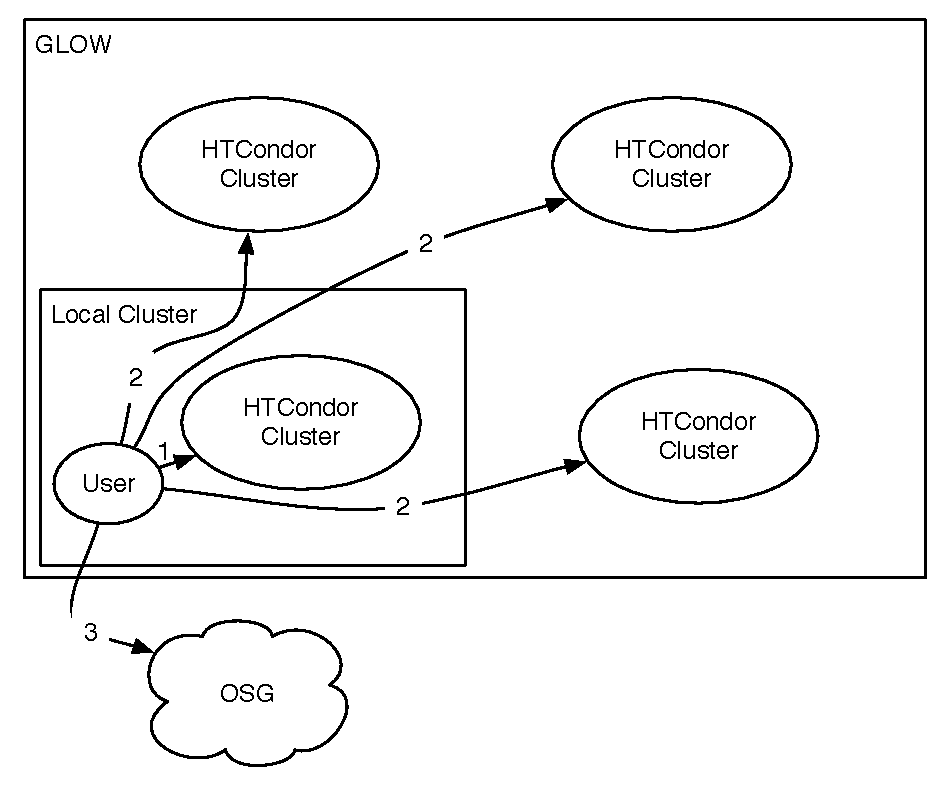
\includegraphics[scale=0.6]{images/GLOW-Campus}
	\caption{Grid Laboratory of Wisconsin Campus Grid}
	\label{fig:GLOWCampus}
\end{figure}


An example of an existing campus grid is the Grid Laboratory of Wisconsin's campus grid.  The Grid Laboratory of Wisconsin (GLOW) \cite{gridworkshopweb, glowwebsite} is a grid at the University of Wisconsin at Madison.  GLOW uses Condor to distribute 
jobs on their campus grid.  A diagram of the campus grid is shown in Figure \ref{fig:GLOWCampus}.  When the user submits a job, it first attempts to run at the local HTCondor cluster.  If the local cluster is unable to meet the demands of the user's jobs, then it attempts to run at HTCondor clusters at the University of Wisconsin.  If they do not meet the demands of the user, the jobs may then run at Purdue's DiaGrid, a regional grid of HTCondor clusters.

Security at the GLOW campus Grid is based on IP whitelisting.  While there is a central 
team available to assist with management, each resource is free to define its own policies and priorities for local 
and remote usage.  Cluster ownership is distributed, although there's also a general-purpose cluster available.  
Software and data are managed by an Andrew File System (AFS) \cite{morris1986andrew} installation and Condor file transfer.  AFS is a global file system
that every worker node will mount, therefore providing a global space to store data and applications.  This simplifies data distribution
by providing a staging area.

The GLOW campus grid is not able to expand to outside resources due to their reliance on a shared file system.  Further, they rely on HTCondor to provide an interface to other clusters.  They are unable to submit to clusters which have other schedulers such as PBS or Slurm.  

%In \cite{weitzel2011campus}, we identified five characteristics of a campus grid:

%\begin{description}
%	\item[Trust Relationships:] A trust relationship enables 
%	a resource provider to grant campus users controlled access to the resource, and may be established through 
%	sociology and/or technology-based security methods.
%	\item[Job Submission:] A method for users to submit processing to the campus grid.
%	\item[Resource Independence:] On a campus, several distinct teams may manage distinct clusters due to campus 
%	organization or ownership.  Management of resources may be divided by college, department, or lab.  One 
%	characteristic of campus grids is the independence of resources--the level of decision-making delegated out to 
%	the resource providers.
%	\item[Accounting:] Accounting may not seem to be an important grid characteristic--it certainly isn't required for 
%	users to successfully run a job.  However, it is critical for the long-term health of the campus grid as it provides a quantitative 
%	measurement of the grid's value.
%	\item[Data Management:] Scientific data management presents  challenges for researchers.  The data volume is often larger than a single scientist can keep on their personal systems, and therefore must use the campus grid's storage resources.
%\end{description}

%The campus grids we have studied in \cite{weitzel2011campus} do not have data management capabilities for large datasets.  

%Grid schedulers have become more popular as the number of resources has increased.  Examples of grid schedulers are OSGMM \cite{website:osgmm} and GlideinWMS \cite{sfiligoi2008glideinwms}.  These schedulers are able to send jobs to remote resources using grid protocols.  OSGMM performs a direct grid submission to the remote resources using the Globus Resource Allocation Manager \cite{foster1999globus} (GRAM)  interface.  GlideinWMS also submits to the GRAM interface of the cluster, but provides an overlay of HTCondor daemons on top of remote resources.  The overlay presents a consistent HTCondor interface to the computing resources for ease of use.  

% Talk about overlays





\section{Data Management}

%There have been previous policy frameworks for distributed storage.  These frameworks have largely been designed to move data between a few large filesystems.  Therefore, the interactions are rare but could make significant changes to the system.  In contrast, the CacheDs have frequent interactions with other agents, but each one has a minimal impact on the entire system.

The previous discussion primarily concerned access to computational resources.  Data management is a further challenge for distributed computing.  For this dissertation, data management can be broken down into three categories: storage systems, transfer protocols, and high level services.  Storage systems provide access to the underlying data storage.  Transfer protocols provide a method to exchange data between storage systems.  High level services provide data management services on top of the file systems, such as data life cycle management, data placement, meta-data storage, and search capabilities.

An example of a data management service is the integrated Rule-Oriented Data System iRODS \cite{rajasekar2010irods}.  It provides meta-data storage, querying, and rule-based placements.  It can perform transfers to storage resources.  When given input, iRODS also has the capability to create rules and take action on data.  It creates a small policy framework that, upon certain actions, can execute micro-services.  Our framework is designed for frequent interaction between many agents acting independently.  The rules for iRODS can be large and cumbersome for simple data replication.  Further, to do anything substantial with the rules, custom code must be written.

iRODS is inflexible in the presence of unreliable underlying storage.  iRODS assumes that any data stored in it is available at any time, and does not periodically check the status of the data it is storing.  This does not make iRODS a good fit for opportunistic storage, which can be unreliable.  

Stork \cite{kosar2004stork} is a data placement scheduler.  It can schedule data placement and transfers to and from remote storage systems.  Stork is innovative in that it treats data transfers similar to jobs.  Just like jobs in a batch system, Stork will queue transfers and check for proper completion of the transfers.  If the transfers fail, it is able to retry the transfers according to policy.  Stork is limited to managing data transfers between storage elements.  It is unable to utilize opportunistic storage resources directly.

Kangaroo \cite{thain2001kangaroo} is another storage scheduler multi-level file access system.  It allows for multiple levels of staging in order to send job output back to a storage device.  It can do this by asynchronously staging data through multiple storage devices on its path to the destination filesystem.  The goal of the Kangaroo system is to utilize unused network and storage resources in order to provide a resilient method for output data transfers.  The Kangaroo system does not attempt to optimize input data transfers.


DQ2 \cite{branco2008managing} and Phedex \cite{rehn2006phedex} are production transfer services for the Atlas and CMS physics experiments, respectively.  They are used to manage distributed transfers to and from sites inside the collaborations.  Additionally, they have had databases built on top of them that provide features such as combining files into datasets for easier bulk transfer management.  Both were designed for their respective physics experiments, and therefore, would be very difficult to generalize for outside users.  Further, both were designed for reliable storage rather than opportunistic storage.

Distributed filesystems such as Hadoop \cite{white2012hadoop} can provide data placement policy.  For example, Hadoop can be configured to replicate the contents of a directory at least $X$ times.  Further, a script can be given to Hadoop which it can query to create a topology of the data center, further providing control of how the data replicas are sent.  This topology script has been used by us to create a data center aware Hadoop replication policy \cite{he2012hog}.

\subsection{Storage Systems}

Distributed file systems have long had their own storage access methods.  An example of this is Hadoop, a popular distributed file and processing system.  The only method to access Hadoop storage is through the Hadoop protocol.  On the Open Science Grid, the primary access methods are through file system independent middleware such as the Storage Resource Manager (SRM) \cite{shoshani2002storage} and XRootd \cite{dorigo2005xrootd}.  They provide a translation layer from system independent grid protocols and security mechanisms to the underlying storage system, such as Hadoop.  The Storage Resource Manager (SRM) is a previously popular protocol to access remote distributed filesystems.  It is a standardized protocol that allows remote, distributed access to large storage with APIs to balance transfers among many data servers.


Beyond storage access methods are storage schedulers.  These schedulers do not define a protocol to access the storage, rather they coordinate the access.  NeST \cite{bent2002flexibility} is a software-only grid aware storage scheduler.  It supports multiple transfer protocols into a storage device, including GridFTP \cite{allcock2005globus} and NFS \cite{walsh1985overview}.  Further, it provides features such as resource discovery, storage guarantees, quality of service, and user authentication.  It is layered over a distributed filesystem to provide access to it.  NeST functions as the interface and access scheduler for a storage device.  Features such as the storage guarantees and quality of service require NeST to be the only interface into the storage device, a very rare feature in today's grid storage.  Today's storage elements, such as the four petabyte Hadoop Distributed Filesystem (HDFS) instance at University of Nebraska--Lincoln, include multiple protocols and interfaces to access the storage element.  Nebraska runs four methods of accessing and modifying storage \cite{attebury2009hadoop}, SRM \cite{shoshani2002storage}, GridFTP, XrootD, and FUSE \cite{szeredi2010fuse} mounted Hadoop.  All of these methods are required for compatibility with different access patterns and clients.  NeST could implement each of these protocols, but it would be extremely difficult to manage the storage centrally.  For example, FUSE is mounted on all 300 worker nodes.  The GridFTP and XrootD servers run on 10s of servers, with an aggregate bandwidth of 10 Gbps.  Scaling quality of service and storage allocation/enforcement across all of these access methods would likely prove impossible.

\subsection{Data Transfer Mechanisms}

Storage systems may exchange data via a number of transfer mechanisms, such as BitTorrent.  BitTorrent has been used for data transfer in computational grids by Wei, Fedak, \& Capello \cite{wei2005collaborative, wei2005scheduling, wei2007towards}.  It has been shown to improve data transfer speeds when compared to traditional source and sink transfer methods, such as FTP \cite{postel1985file}, the base protocol to GridFTP, a grid enabled FTP protocol.  The researchers did not compare performance of the BitTorrent protocol when compared to modern grid transfer techniques, such as using HTTP caching.  Further, the authors did not test BitTorrent transfers across diverse network topologies that are common on the grid.  A worker node from one cluster may not be able to communicate directly with a worker node from another cluster.  Therefore, BitTorrent may not work between clusters but will work inside clusters.

Globus Online \cite{foster2011globus} is a web interface for transferring files between sites and sharing data with other users.  It offers an intuitive web interface for bulk transfers between endpoints.  It only supports the GridFTP \cite{allcock2005globus} transfer protocol and requires GridFTP implementations at all endpoints.

There are also popular data transfer tools used on clusters such as secure copy (SCP) from OpenSSH \cite{openssh} and rsync \cite{rsynce}.  SCP is a simple copy tool that uses the Secure Shell (SSH) protocol to transfer files from a source to a client.  Rsync is also able to copy files from a source to a client, but it can also do differential copies, where only the changed portion of a directory will be copied at a time.  Both of these methods are used heavily when the data size is small.  But they both use single stream TCP in order to transfer data, which in practice has been shown to be slower than multiple TCP streams as used in GridFTP \cite{allcock2005globus} or BitTorrent.



\begin{figure}[ht!]
	\centering
	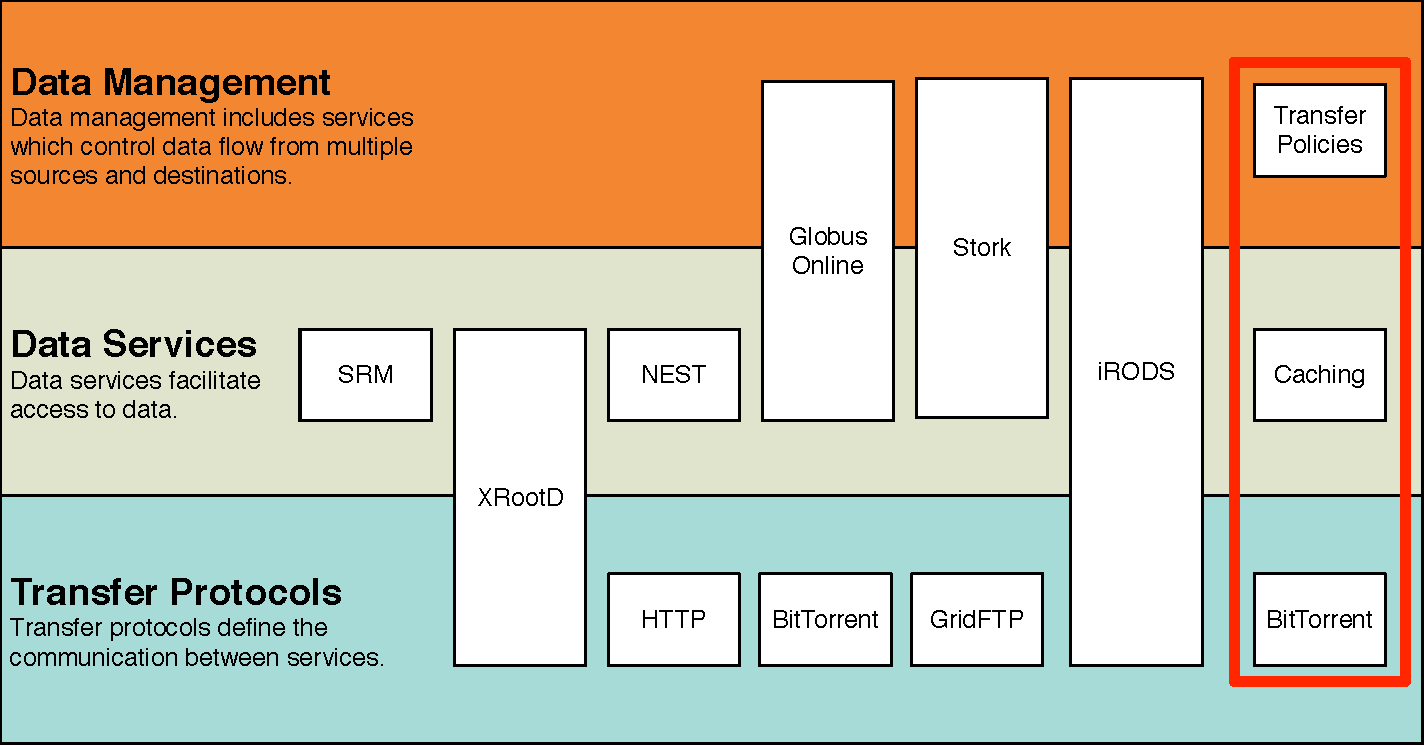
\includegraphics[width=\textwidth]{images/BackgroundStorageDiagram2.pdf}
	\caption{Storage Technology Categorization}
	\label{fig:backgroundstorage}
\end{figure}

Figure \ref{fig:backgroundstorage} shows an overview of the different protocols and services, and how they fit into the three categories: Data Management, Data Services, and Transfer Protocols.

\section{State of Practice in Campus Computing}
\label{sec:currentapproach}
In order to illustrate the available technologies on the grid, we will begin with a common user application.  We will then describe the technologies that could enable this computing on the grid.

\subsection{Use Case}
We will focus on the use of a commonly used biology application, BLAST \cite{altschul1990basic}.  BLAST workflows typically include the following files:

\begin{itemize}
	\item \textbf{Executable:} The BLAST application is distributed with many executables, such as \texttt{blastp} and \texttt{blastx}.  They are run on the remote execution resources and produce output.  In this dissertation, we will be primarily using \texttt{blastp}, which searches protein sequences.
	\item \textbf{Database:}  A large listing of sequences that will be scanned for similarities to the sequences in the query files.
	\item \textbf{Query Files:} A small list of sequences that will be compared to the sequences in the database to find similarities.  
\end{itemize}

\begin{figure}
	\centering
	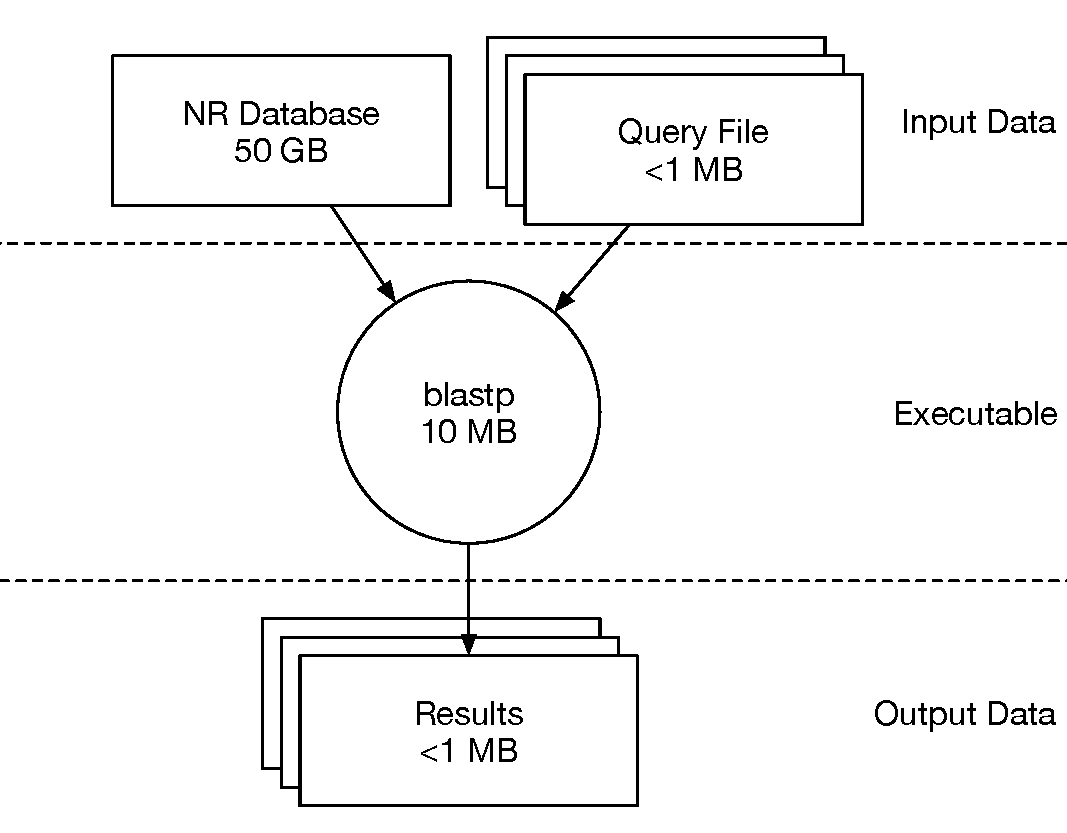
\includegraphics[width=0.7\textwidth]{images/BlastWorkflow}
	\caption{Blast Workflow}
	\label{fig:blastworkflow}
\end{figure}

Each of these files have different properties.  The executable is relatively small, often 10s of megabytes, but identical copies are used by all executions of BLAST.  The query files are unique to each job but are typically very small, not exceeding 1 MB.  The database is a large collection of proteins that is searched for each protein in the query file.  Many databases are publicly available for use in BLAST.  The most common is the non-redundant (NR) database, which is currently 50 GB and updated weekly.  A diagram of the workflow is shown in Figure \ref{fig:blastworkflow}.

\subsection{Current Approach}


If the user has a BLAST application and wishes to run numerous jobs, they must first gain access to computational resources.  They may have access to a campus cluster.  In that case, they will login to the campus cluster.  The first step for the user is to learn the scheduler language.  There are many different languages, such as PBS, Slurm, or HTCondor; all  have slightly different syntax.

Once the scheduler language has been learned enough to write a submission file, the data must be transferred to the cluster from their laptop.  This is usually accomplished with a tool such as SCP from the OpenSSH \cite{openssh} package.  This will be transferred slowly as SCP only uses a single encrypted stream to send data.  The 50 GB NR database, transferred from the user's wireless connected laptop to the cluster could take two hours (at 54 Mbps), if nothing goes wrong with the transfer.

Once the data is on the cluster, the user will submit the jobs to the scheduler to process the data.  The BLAST database will be copied for each and every execution to the execution resources from the cluster's shared filesystem.

Once the computation has completed, the user will copy the output data back to their laptop for further analysis.

\subsection{Issues with Current Approach}

There are many issues with the current approach:

\begin{itemize}
	\item Users must learn one or more scheduler languages.  If users want to submit to only one cluster, then they only need to learn one submission language.  But if their demands grow, and they need more resources, they will need to learn another programming language.
	\item Data copies are very expensive and should be minimized.  The NR database is updated frequently;  therefore, it must be updated on the cluster frequently.
	\item Once on the cluster, each job will need to copy the NR database to the worker node in order to process it, even if was already copied by a previous job.  This copy will happen every time, as there is no caching in the vast majority of distributed filesystems.
\end{itemize}







